%COLORS
%reds
\definecolor{cus-red}{RGB}{	254, 82, 88}
\definecolor{cus-red1}{RGB}{241, 14, 22}
\definecolor{cus-red2}{RGB}{251,62,4}
%blues
\definecolor{cus-blue}{RGB}{82, 203, 254}
\definecolor{cus-blue1}{RGB}{14, 173, 241}
\definecolor{cus-blue2}{RGB}{9, 115, 161}
\definecolor{cus-blue3}{RGB}{4,111,251}
%oranges
\definecolor{cus-orange}{RGB}{254, 134, 82}
\definecolor{cus-orange1}{RGB}{254, 144, 4}

\definecolor{cus-sky}{RGB}{85,213,255}
\definecolor{cus-green}{RGB}{29,181,97}
\definecolor{cus-aqua}{RGB}{91, 236, 221}
\definecolor{cus-purp}{RGB}{178, 89, 238}

\definecolor{cus-yellow}{RGB}{254, 191, 82}
\definecolor{cus-green1}{RGB}{148, 238, 89}
\definecolor{cus-violet}{RGB}{148, 238, 89}
\definecolor{branches}{RGB}{147, 98, 1}
\definecolor{cus-tur}{RGB}{9, 161, 156}
\definecolor{cus-white}{RGB}{250,250,250}
\definecolor{cus-black}{RGB}{111,113,114}

%TRIANGLE OBJECTS


\newcommand{\circtri}[1]{
	
	\begin{scope}[xshift=#1 cm]
		\foreach \x in {-8,-7.95,...,7}{
			\foreach \c in { cus-blue,cus-red,cus-orange,cus-yellow,cus-blue1,cus-red1,cus-green,
				cus-aqua,cus-purp,cus-blue2,cus-green1,cus-violet}{
				\draw [thick,rotate=rand*360,xshift=\x*.6 cm,fill=\c,scale=\x*.1] (0 ,0)--(1 ,2)--(2 ,0) -- cycle; 	
			}
		}
	\end{scope}
}
	
\newcommand{\triforce}[5]{
	\begin{scope}[xshift=#1 cm, yscale=#2,yshift=#5 cm]
		\draw [thick,red,fill=#3] (0 ,0)--(1,1.73)--(2 ,0) -- cycle; 
		\draw [thick,rotate around ={60:(0 ,0)},fill=#4] (0 ,0)--(1,1.73)--(2 ,0) -- cycle; 
		\draw [thick,rotate around ={60:(1 ,1.73)},fill=#4] (0 ,0)--(1,1.73)--(2 ,0) -- cycle; 
		\draw [thick,rotate around ={60:(2 ,0)},fill=#4] (0 ,0)--(1,1.73)--(2 ,0) -- cycle;	
\end{scope}
}
\newcommand{\tritile}[1]{
	\begin{scope}[scale=#1]
	\foreach \x in {-10,-6,...,6}{
		\foreach \y in {6,2.5,-1,...,-15}{
			\triforce{\x}{1}{black}{cus-purp}{\y}
		}
	}
	\foreach \x in {-8,-4,...,4}{
		\foreach \y in {-6,-2.5,...,15}{
			
			\triforce{\x}{-1}{black}{cus-orange}{\y}
		}
	}
	\end{scope}
}
\newcommand{\hexagon}[5]{
	\begin{scope}[xshift = #1 cm, yshift = #2 cm,rotate = #5]
		\foreach \c [count=\r from 1] in {#3,#4,#3,#4,#3,#4}{
			\draw [thick,rotate around ={\r*60:(0 ,0)},fill=\c] (0 ,0)--(1,1.73)--(2 ,0) -- cycle; 
		}
\end{scope}
}

\newcommand{\pentagon}[5]{
	\begin{scope}[xshift = #1 cm, yshift = #2 cm, rotate = #5]
		\foreach \c [count=\r from 1] in {#3,#4,#3,#4,#3}{
			\draw [thick,rotate around ={\r*72:(0 ,0)},fill=\c] (0 ,0)--(1,1.73)--(2 ,0) -- cycle; 
		}
\end{scope}}

\newcommand{\qua}[5]{
	\begin{scope}[xshift = #1 cm, yshift = #2 cm, rotate = #5]
		\foreach \c [count=\r from 1] in {#3,#4,#3,#4}{
			\draw [thick,rotate around ={\r*90:(0 ,0)},fill=\c] (0 ,0)--(1,1.73)--(2 ,0) -- cycle; 
		}
\end{scope}
}

\newcommand{\tri}[5]{
	\begin{scope}[xshift = #1 cm, yshift = #2 cm, rotate = #5]
		\foreach \c [count=\r from 1] in {#3,#4,#3}{
			\draw [thick,rotate around ={\r*120:(0 ,0)},fill=\c] (0 ,0)--(1,1.73)--(2 ,0) -- cycle; 
		}
\end{scope}
}

\newcommand{\duo}[5]{
	\begin{scope}[xshift = #1 cm, yshift = #2 cm, rotate = #5]
		\foreach \c [count=\r from 1] in {#3,#4}{
			\draw [thick,rotate around ={\r*180:(0 ,0)},fill=\c] (0 ,0)--(1,1.73)--(2 ,0) -- cycle; 
		}
	\end{scope}
}

%TABLE OBJECTS


\newcommand{\ntwo}{
	
	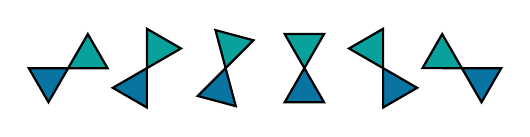
\begin{tikzpicture}
	\begin{scope}[scale = .25]
	\foreach \r [count=\x from 1] in {0,30,45,60,90,120}{
		\duo{\x*4}{0}{cus-blue2}{cus-tur}{\r}
	}
	\end{scope}
	
	\end{tikzpicture}
}


\newcommand{\nthree}{
	
	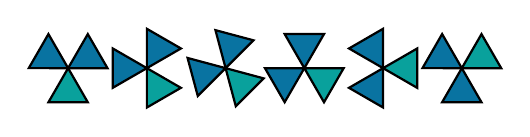
\begin{tikzpicture}
	\begin{scope}[scale = .25]
	\foreach \r [count=\x from 1] in {0,30,45,60,90,120}{
		\tri{\x*4}{0}{cus-blue2}{cus-tur}{\r}
	}
	\end{scope}
	
	\end{tikzpicture}
}

\newcommand{\nfour}{
	
	
\begin{tikzpicture}
	\begin{scope}[scale = .25]
	\foreach \r [count=\x from 1] in {0,30,45,60,90,120}{
		\qua{\x*4}{0}{cus-blue2}{cus-tur}{\r}
	}
	\end{scope}
	
	\end{tikzpicture}
}

\newcommand{\nfive}{
	
	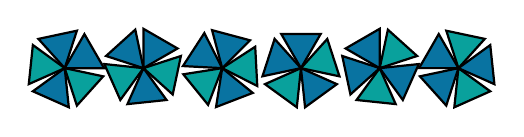
\begin{tikzpicture}
	\begin{scope}[scale = .25]
	\foreach \r [count=\x from 1] in {0,30,45,60,90,120}{
		\pentagon{\x*4}{0}{cus-blue2}{cus-tur}{\r}
	}
	\end{scope}
	
	\end{tikzpicture}
}

\newcommand{\nsix}{
	
	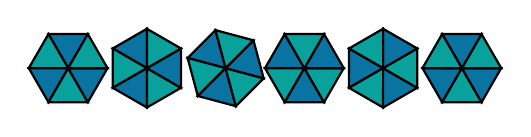
\begin{tikzpicture}
	\begin{scope}[scale = .25]
	\foreach \r [count=\x from 1] in {0,30,45,60,90,120}{
		\hexagon{\x*4}{0}{cus-blue2}{cus-tur}{\r}
	}
	\end{scope}
	
	\end{tikzpicture}
}

%%%%%%%%%%%%%%%%%%%%%%%%%%%%%%%%%%%%%%%%%%%%%%%%%%%%%%%%%%%%%%%%%%%%%%%%%%%%%%%%%%%%
%Pattern Objects
\newcommand{\single}[1]{
	
	\begin{tikzpicture}
	\draw [thick,fill=#1] (0 ,0)--(1,1.73)--(2 ,0) -- cycle;
\end{tikzpicture}
}
\newcommand{\tduo}[7]{
\begin{tikzpicture}[scale = #1,background rectangle/.style={fill=#5}, show background rectangle]
\foreach \x in {#2}{
	\foreach \y in {#3}{
		\duo{\x}{\y}{#6}{#7}{#4}
	}	
}

\end{tikzpicture}
}


\newcommand{\trio}[7]{
	
\begin{tikzpicture}[scale = #1,background rectangle/.style={fill=#5}, show background rectangle]

\foreach \x in {#2}{
	\foreach \y in {#3}{
		\tri{\x}{\y}{#6}{#7}{#4}
	}	
}

\end{tikzpicture}
}
 
\newcommand{\quadr}[7]{
	\begin{tikzpicture}[scale = #1,background rectangle/.style={fill=#5}, show background rectangle]
		\foreach \x in {#2}{
			\foreach \y in {#3}{
				\qua{\x}{\y}{#6}{#7}{#4}
			}	
		}
	\end{tikzpicture}
}
\newcommand{\pent}[7]{
\begin{tikzpicture}[scale = #1,background rectangle/.style={fill=#5}, show background rectangle]
	\foreach \x in {#2}{
		\foreach \y in {#3}{
			\pentagon{\x}{\y}{#6}{#7}{#4}
		}	
	}
\end{tikzpicture}
}
\newcommand{\hex}[7]{
	\begin{tikzpicture}[scale = #1,background rectangle/.style={fill=#5}, show background rectangle]
		\foreach \x in {#2}{
			\foreach \y in {#3}{
				\hexagon{\x}{\y}{#6}{#7}{#4}
			}	
		}
	\end{tikzpicture}
}